\documentclass[11pt]{article}
\usepackage[margin=1in]{geometry}
\usepackage{amsmath,amssymb,amsthm}
\usepackage{booktabs}
\usepackage[colorlinks=false,pdfborder={0 0 0}]{hyperref}
\usepackage{enumitem}
\usepackage{graphicx}
\usepackage{algorithm}
\usepackage{algorithmic}
% \usepackage{multirow}

\newtheorem{definition}{Definition}
\newtheorem{proposition}{Proposition}
\newtheorem{theorem}{Theorem}
\newtheorem{remark}{Remark}
\newtheorem{corollary}{Corollary}

\title{Computational Primes:\\A Systematic Framework for Partitioning\\Neural Network Computation Across\\Analog and Digital Domains}
\author{Michael Bieg\\
\textit{Independent Researcher}\\
\texttt{Bieg.Michael@web.de}}
\date{July 2026 (v2)}

\begin{document}
\maketitle

\begin{abstract}
Analog and mixed-signal neural network accelerators face a universal design problem: which operations should be computed in the analog domain (exploiting physics at near-zero energy cost) and which should remain digital (exact but energy-intensive)? Current approaches solve this partitioning problem ad hoc for each chip design. We introduce \textbf{Computational Primes}---a set of 12 irreducible operations with known physical implementations (P1--P12) and 4 operations without physical equivalents (X1--X4)---and show that every neural network algorithm can be factored into these primes. This factorization enables a systematic compiler that (1)~decomposes any compute graph into primes, (2)~assigns each prime to the analog or digital domain based on hardware constraints, (3)~identifies multi-computation fusion opportunities where a single physical event yields multiple outputs, and (4)~minimizes domain transitions (ADC/DAC). We factorize 107 algorithms spanning transformer inference, training, generative models, reinforcement learning, GNNs, and SSMs. Of these, 79 are fully mappable to analog hardware, 22 become mappable on GPUs (where X2 and X4 are available), and 6 remain fundamentally unmappable. Analysis of five recent analog chips (IBM 14nm PCM, TSMC CIM, Extropic XTR-0, Normal Computing CN101, J\"ulich gain-cell) shows that all made suboptimal manual partitioning decisions that the prime compiler would have improved. We further demonstrate that RMSNorm---used by LLaMA, Mistral, and Gemma---has a fully analog implementation via AGC feedback circuits, resolving the last major open mapping for transformer inference. New in v2, we validate this claim at circuit level with 602 SPICE simulations: the AGC feedback loop settles to the exact RMSNorm equilibrium within 4--6~ns and, crucially, is structurally robust to device mismatch, whereas the open-loop translinear pipeline---mathematically exact with ideal junctions ($<\!10^{-6}$ relative error)---degrades to 1.5--4.5 effective bits under realistic mismatch. Feedback, not open-loop translinear arithmetic, is the viable path to analog normalization.
\end{abstract}

\section{Introduction}

The past three years have seen an unprecedented surge in analog and mixed-signal neural network accelerators. IBM demonstrated a 14nm PCM chip running ALBERT~\cite{ibm2025}, TSMC fabricated a memristor+SRAM heterogeneous CIM processor~\cite{tsmc2025}, Extropic built a thermodynamic computing board for diffusion models~\cite{extropic2025}, Normal Computing taped out an RLC-based sampling ASIC~\cite{normal2025}, and Leroux et al.\ at Forschungszentrum J\"ulich showed analog attention with 70,000$\times$ energy reduction over GPUs~\cite{leroux2025a}.

Every one of these projects confronted the same fundamental question: \textit{Which operations should be computed in the analog domain, and which should remain digital?}

Currently, each team answers this question through manual analysis specific to their hardware and target workload. IBM maps matrix multiplications to PCM crossbars but keeps LayerNorm and Softmax digital. Leroux et al.\ replace Softmax with HardSigmoid because ``normalization operations are challenging to implement using analog circuitry''~\cite{leroux2025a}. No systematic framework exists for making these decisions.

We introduce such a framework. Our contributions are:

\begin{enumerate}[leftmargin=*]
\item \textbf{Computational Primes}: A catalog of 12 irreducible operations (P1--P12) with verified physical implementations and 4 operations (X1--X4) without physical equivalents, forming a complete basis for neural network computation (\S\ref{sec:primes}).

\item \textbf{Universal factorization}: Decomposition of 107 algorithms into their prime factors, enabling immediate assessment of analog mappability (\S\ref{sec:factorization}).

\item \textbf{Domain assignment and fusion}: A decision framework for analog/digital partitioning with automatic detection of multi-computation opportunities---physical events that yield $2$--$12\times$ throughput multipliers at zero marginal hardware cost (\S\ref{sec:compiler}).

\item \textbf{RMSNorm resolution}: The first fully analog mapping of RMSNorm via automatic gain control (AGC) feedback, eliminating the last major barrier to fully analog transformer inference (\S\ref{sec:rmsnorm}).

\item \textbf{Circuit-level validation (new in v2)}: SPICE simulations (602 runs, real junction $I$--$V$ characteristics, Monte-Carlo device mismatch) confirming the AGC mapping and quantifying \textit{why} it wins: feedback converts per-device mismatch into a harmless common-mode gain error, while the open-loop translinear pipeline accumulates per-channel distortion (\S\ref{sec:validation}).

\item \textbf{Chip analysis}: Retrospective analysis of five recent analog chips showing that prime-compiler-guided partitioning would have captured 15--40\% additional energy savings on nonlinear operations (\S\ref{sec:analysis}).
\end{enumerate}

\subsection{Scope and Limitations}

This is a \textit{framework} paper, not a chip paper. We do not fabricate hardware or claim measured speedups. The value is in the systematic methodology: replacing ad hoc partitioning decisions with a principled, automatable approach. All quantitative claims about analog implementations reference published, peer-reviewed hardware results. New in v2, the RMSNorm mapping (\S\ref{sec:rmsnorm}) is additionally validated by circuit simulation at a defined intermediate fidelity---junction-exact device equations with idealized loop wiring (\S\ref{sec:validation})---which quantifies mismatch sensitivity but does not replace silicon measurement.

\section{Computational Primes}
\label{sec:primes}

\begin{definition}[Computational Prime]
An operation $P$ is a computational prime if (a)~it cannot be decomposed into simpler operations that each have independent physical implementations, and (b)~it has at least one verified mapping to a physical system that computes it at $O(0)$ marginal energy cost.
\end{definition}

We identify 12 primes satisfying this definition (Table~\ref{tab:primes}) and 4 ``missing primes'' that lack any known physical implementation (Table~\ref{tab:missing}).

\subsection{The 12 Physical Primes}

\begin{table}[t]
\centering
\caption{The 12 computational primes with physical implementations.}
\label{tab:primes}
\footnotesize
\begin{tabular}{clllll}
\toprule
ID & Operation & Symbol & Physics & Hardware & Ref. \\
\midrule
P1 & Accumulation & $\Sigma$ & Kirchhoff's Current Law & Wire junction & \cite{prezioso2015} \\
P2 & Scaling & $\times c$ & Ohm's Law: $I = G \cdot V$ & Memristor / resistor & \cite{prezioso2015} \\
P3 & Exponential & $e^x$ & Boltzmann: $P \propto e^{-E/kT}$ & sMTJ / subthreshold FET & \cite{bieg2025,sillman2023} \\
P4 & Logarithm & $\ln x$ & Diode: $V = \frac{kT}{q}\ln\frac{I}{I_s}$ & Diode / subthreshold FET & \cite{tageldeen2025} \\
P5 & Selection & $\arg\max$ & Race to threshold & sMTJ array / WTA & \cite{bieg2025,bieg2026} \\
P6 & Sigmoid & $\sigma(x)$ & Fermi-Dirac distribution & Subthreshold FET pair & \cite{mram_sigmoid2022} \\
P7 & Threshold & $\theta(x)$ & Phase transition / comparator & Schmitt trigger & --- \\
P8 & Integration & $\int$ & Charge: $Q = \int I\,dt$ & Capacitor / memristor & \cite{denram2024} \\
P9 & Differentiation & $d/dt$ & Induction: $V = L\frac{dI}{dt}$ & RC high-pass & --- \\
P10 & Stochasticity & $\xi$ & Thermal fluctuation & Johnson-Nyquist / RTN & \cite{cryptoristor2024} \\
P11 & Multiplication & $a \times b$ & Transistor square law & Gilbert cell & --- \\
P12 & Inversion & $1/x$ & Translinear loop & BJT/MOSFET circuit & \cite{tageldeen2025} \\
\bottomrule
\end{tabular}
\end{table}

\textbf{P1 (Accumulation, $\Sigma$):} $y = \sum_i x_i$. Kirchhoff's Current Law guarantees that currents sum at any node. Cost: $O(0)$---charge conservation is exact and requires no energy.

\textbf{P2 (Scaling, $\times c$):} $y = c \cdot x$. Ohm's Law: $I = G \cdot V$ where the conductance $G$ encodes the constant $c$. In memristive crossbars, P1$\cdot$P2 = matrix-vector multiplication.

\textbf{P3 (Exponential, $e^x$):} Any MOSFET in the subthreshold regime: $I_D = I_0 \exp(V_{GS}/nV_T)$. Also realized via Arrhenius rates in sMTJs~\cite{bieg2025} and chemical kinetics~\cite{bieg2026}.

\textbf{P4 (Logarithm, $\ln x$):} The inverse of P3. A diode's voltage is $V = (kT/q)\ln(I/I_s)$. Precision limited by ideality factor $n$ (typically 1.0--1.5); \S\ref{sec:validation} quantifies how ideality \textit{mismatch} between devices propagates through log-domain arithmetic.

\textbf{P5 (Selection, $\arg\max$):} A race among competing exponential processes: the first to fire identifies the maximum. Produces exact softmax samples in $O(1)$ time~\cite{bieg2025}. The race simultaneously yields 5 additional observables~\cite{bieg2026}.

\textbf{P6 (Sigmoid, $\sigma$):} The Fermi-Dirac distribution $f(E) = 1/(1 + e^{(E-\mu)/kT})$ is natively computed by a subthreshold MOSFET transfer characteristic. Variants: $\tanh(x) = 2\sigma(2x) - 1$.

\textbf{P7 (Threshold, $\theta$):} A comparator or Schmitt trigger implements $y = 1$ if $x > 0$, else $0$. In the Ising model limit ($T \to 0$), this is a phase transition.

\textbf{P8 (Integration, $\int$):} Charge accumulation on a capacitor: $Q = \int I\,dt$. Volatile (capacitor, $\tau \propto RC$) or non-volatile (memristor, floating gate). DenRAM~\cite{denram2024} demonstrated programmable RC time constants for temporal processing.

\textbf{P9 (Differentiation, $d/dt$):} An RC high-pass filter or inductor: $V = L\,dI/dt$. Passive circuit, $O(0)$ cost. Limited by noise amplification at high frequencies.

\textbf{P10 (Stochasticity, $\xi$):} Thermal fluctuations generate true randomness at zero cost. Johnson-Nyquist noise ($V^2 = 4kTR\Delta f$), sMTJ random switching, or random telegraph noise in standard MOSFETs~\cite{cryptoristor2024}. Normally suppressed; here exploited.

\textbf{P11 (Variable Multiplication, $\times$):} $y = a \cdot b$ where both inputs are variables. The Gilbert cell (4-quadrant analog multiplier) computes this via the transistor square law. Distinct from P2 (one input is a stored constant).

\textbf{P12 (Inversion, $1/x$):} Translinear loops~\cite{gilbert1975} compute $I_{out} = I_a \cdot I_b / I_c$ using 4--6 BJTs or subthreshold MOSFETs. Derived operations: $\sqrt{x}$ (feedback loop), $x^\alpha$ (cascaded loops), $1/\sqrt{x}$ (combination). As \S\ref{sec:validation} shows, P12 realized \textit{open-loop} is mismatch-fragile; realized \textit{implicitly through feedback equilibrium} it is robust.

\subsection{The 4 Missing Primes}

\begin{table}[h]
\centering
\caption{Missing primes: no known physical implementation.}
\label{tab:missing}
\begin{tabular}{clcc}
\toprule
ID & Operation & Analog & GPU \\
\midrule
X1 & Symbol manipulation & $\times$ & $\times$ \\
X2 & Dynamic topology & $\times$ & $\checkmark$ \\
X3 & Unbounded recursion & $\times$ & $\sim$ \\
X4 & Symbolic tracing & $\times$ & $\checkmark$ \\
\bottomrule
\end{tabular}
\end{table}

\textbf{X1 (Symbol, SYM):} Rule-based discrete symbol processing (BPE tokenization, regex, hashing). No continuous numerical structure $\Rightarrow$ no physical mapping. Blocks: tokenizer, graph isomorphism.

\textbf{X2 (Dynamic Topology, DYN):} Runtime reconfiguration of connectivity. Analog hardware has fixed wiring. On GPUs: warp schedulers, shared memory addressing. Blocks (analog): KV-cache eviction, experience replay.

\textbf{X3 (Unbounded Recursion, REC):} Data-dependent recursion depth requires unbounded memory. Physical hardware is finite. GPU stack limited to ${\sim}1024$ frames. Blocks: MCTS.

\textbf{X4 (Symbolic Tracing, TAPE):} Recording the compute graph for reverse-mode differentiation. Requires a meta-level. On GPUs: CUDA Graphs, \texttt{torch.compile}. Blocks (analog): backpropagation.

\subsection{Completeness of the Prime Basis}
\label{sec:completeness}

\begin{proposition}[Completeness]
Every differentiable function $f: \mathbb{R}^n \to \mathbb{R}^m$ computable on digital hardware can be expressed as a composition of primes P1--P12 and X1--X4.
\end{proposition}

\begin{proof}[Proof sketch]
P1--P4 and P11--P12 form a complete basis for arithmetic ($+, -, \times, \div, \exp, \ln$). P6 and P7 provide nonlinear activation. P5 provides selection. P8--P9 provide temporal dynamics. P10 provides stochasticity. X1--X4 cover discrete/symbolic operations outside continuous arithmetic. Any algorithm is a directed acyclic graph of these primitives. A fully rigorous treatment---a formal operational semantics for the prime composition algebra---is beyond the scope of this paper. \qed
\end{proof}

Factorizations are generally \textit{not} unique. Squaring, for example, can be realized directly (P11 in self-multiply mode) or in the log domain as P3$\cdot$P2$\cdot$P4---the validation testbench of \S\ref{sec:validation} exploits exactly this freedom. Version~1 of this paper claimed uniqueness up to commutativity; that claim was too strong. Non-uniqueness is in fact a feature, not a defect: the set of admissible factorizations of an operation is precisely the search space over which the compiler's domain-assignment phase (\S\ref{sec:compiler}) optimizes, choosing the realization whose primes best match the target hardware.

\section{Factorization of Neural Network Algorithms}
\label{sec:factorization}

\begin{table}[t]
\centering
\caption{Prime factorization of 107 algorithms (subset; full table in supplement). \textbf{M} = mappable, \textbf{G} = GPU-mappable, \textbf{U} = unmappable.}
\label{tab:factorizations}
\footnotesize
\begin{tabular}{rllcl}
\toprule
\# & Algorithm & Factorization & Status & Blocker / Note \\
\midrule
\multicolumn{5}{l}{\textit{Transformer / LLM Core}} \\
1 & RMSNorm & P1$\cdot$P2$\cdot$P11$\cdot$P12 & \textbf{M} & \textbf{Solved}: AGC feedback (\S\ref{sec:rmsnorm}, validated \S\ref{sec:validation}) \\
2 & GELU/SiLU & P11$\cdot$P6 & \textbf{M} & Solved: RRAM Swish~\cite{rram_swish2022} \\
3 & RoPE & P11$\cdot$P2 & \textbf{M} & Fixed trig.\ coefficients \\
4 & KV-Cache+Eviction & P8$\cdot$P5 + X2 & \textbf{G} & Dynamic addressing \\
5 & Causal Masking & P5$\cdot$P7 & \textbf{M} & Solved: race topology~\cite{bieg2025} \\
6 & Multi-Head Split & P2$\cdot$P1 & \textbf{M} & Parallel crossbars \\
7 & Residual Connection & P1 & \textbf{M} & Solved: KCL~\cite{bieg2025} \\
8 & Token Embedding & P8$\cdot$P2 & \textbf{M} & Crossbar; area scales with vocab \\
\midrule
\multicolumn{5}{l}{\textit{Training \& Optimization}} \\
9 & Backpropagation & P11$\cdot$P1$\cdot$P9 + X4 & \textbf{G} & Graph tracing \\
10 & Adam/AdamW & P1$\cdot$P2$\cdot$P11$\cdot$P12$\cdot$P8 & \textbf{M} & $3\times$param storage; impractical at scale \\
13 & Cross-Entropy Loss & P3$\cdot$P4$\cdot$P1$\cdot$P2 & \textbf{M} & Solved: race+diode~\cite{bieg2025} \\
\midrule
\multicolumn{5}{l}{\textit{Generative Models}} \\
14 & Diffusion Reverse & P3$\cdot$P1$\cdot$P2$\cdot$P10$\cdot$P11 & \textbf{M} & $T$ serial passes; solved: DTCA~\cite{extropic2025} \\
15 & VAE Reparametrization & P1$\cdot$P2$\cdot$P10 & \textbf{M} & Solved: DC + noise~\cite{bieg2025} \\
\midrule
\multicolumn{5}{l}{\textit{Sequence Models}} \\
28a & S4D (time-invariant SSM) & P8$\cdot$P2$\cdot$P1 & \textbf{M} & Solved: memristor CIM~\cite{zhang2025ssm} \\
28b & Mamba (selective SSM) & P8$\cdot$P2$\cdot$P1$\cdot$P11 + X2 & \textbf{G} & Input-dep.\ weight reprogramming \\
30 & MoE Routing & P5$\cdot$P1$\cdot$P2$\cdot$P3 & \textbf{M} & Top-K race~\cite{bieg2025} \\
39 & Top-K Sampling & P5$\cdot$P3 & \textbf{M} & Solved: K-fold race~\cite{bieg2026} \\
\midrule
\multicolumn{5}{l}{\textit{Fundamentally Unmappable}} \\
23 & MCTS & P5$\cdot$P10 + X2$\cdot$X3 & \textbf{U} & Unbounded tree \\
26 & WL-Test / Graph Iso & X1 & \textbf{U} & Symbolic hashing \\
38 & BPE Tokenizer & X1 & \textbf{U} & No continuous structure \\
\bottomrule
\end{tabular}
\end{table}

We factorize 107 algorithms into their prime components (Table~\ref{tab:factorizations} shows a representative subset; the full table with all 107 algorithms is in the supplement). Where multiple factorizations exist (\S\ref{sec:completeness}), the table lists the canonical lowest-depth one. The factorization follows a consistent methodology:

\begin{enumerate}[leftmargin=*]
\item Decompose the algorithm into elementary operations (addition, multiplication, exponentiation, comparison, etc.).
\item Map each elementary operation to the corresponding prime.
\item Identify missing primes (X1--X4) that block analog mapping.
\item Classify: \textbf{M}appable (all primes physical), \textbf{G}PU-mappable (X2/X4 available), or \textbf{U}nmappable (X1 or X3 required).
\end{enumerate}

\textbf{Summary}: Of 107 algorithms, 79 are fully mappable to analog hardware, 22 become mappable on GPUs where X2 (dynamic topology) and X4 (symbolic tracing) are available, and 6 are fundamentally unmappable due to X1 (symbol manipulation) or X3 (unbounded recursion).

\section{The Prime Compiler}
\label{sec:compiler}

The prime compiler takes a compute graph and a hardware specification as input and produces an optimally partitioned execution plan.

\subsection{Phase 1: Prime Annotation}

Given a compute graph $G = (V, E)$ (e.g., from \texttt{torch.fx} or ONNX), each node $v \in V$ is annotated with its prime factorization:

\begin{algorithmic}
\STATE \textbf{function} \textsc{Annotate}($v$)
\STATE \quad $\textit{primes}(v) \gets \textsc{Factorize}(v.\textit{op})$
\STATE \quad \textbf{for each} $p \in \textit{primes}(v)$ \textbf{do}
\STATE \quad \quad $\textit{domain}(v, p) \gets \textsc{undecided}$
\STATE \quad \textbf{end for}
\end{algorithmic}

The factorization rules (Table~\ref{tab:factorizations}) are stored as a pattern-matching table. Unknown operations are flagged for manual decomposition.

\subsection{Phase 2: Domain Assignment}

For each prime instance, the compiler decides: \textsc{physics} (analog, $O(0)$ energy, noisy) or \textsc{digital} (exact, energy-intensive).

\begin{definition}[Domain Assignment Problem]
Given annotated graph $G$ with primes $\{p_1, \ldots, p_m\}$ and hardware profile $H$ specifying per-prime analog feasibility, noise tolerance, and transition costs, find the assignment $\delta: \{p_1, \ldots, p_m\} \to \{\textsc{physics}, \textsc{digital}\}$ minimizing total cost:
\begin{equation}
C(\delta) = \sum_{p_i: \delta(p_i)=\textsc{dig}} E_{\textsc{dig}}(p_i) + \sum_{\textsc{transitions}} E_{\textsc{adc/dac}}
\end{equation}
subject to output accuracy constraints.
\end{definition}

The decision is guided by a per-prime feasibility matrix (Table~\ref{tab:assignment}).

\begin{table}[h]
\centering
\caption{Domain assignment heuristic per prime.}
\label{tab:assignment}
\small
\begin{tabular}{clll}
\toprule
Prime & Physics if\ldots & Digital if\ldots \\
\midrule
P1 $\Sigma$ & fan-in $< 256$ & fan-in $> 1000$ \\
P2 $\times c$ & variability $<$ tolerance & precision $> 8$b \\
P3 $e^x$ & range $< 10$ decades & extreme range \\
P4 $\ln$ & diode/BJT available (subthreshold) & $> 2$ decade range \\
P5 $\top$ & always physics & --- \\
P6 $\sigma$ & $kT/q$ slope matches & exact slope needed \\
P7 $\theta$ & always physics (comparator/Schmitt) & --- \\
P8 $\int$ & capacitor available ($\tau$ in range) & long time constants \\
P9 $d/dt$ & RC differentiator available & precision required \\
P10 $\xi$ & always physics & --- \\
P11 $\times$ & THD $<$ tolerance & linearity $> 1\%$ \\
P12 $1/x$ & \textit{in feedback loop}, or trimmed open-loop & open-loop, untrimmed (\S\ref{sec:validation}) \\
\bottomrule
\end{tabular}
\end{table}

\subsection{Phase 3: Multi-Computation Fusion}

After domain assignment, the compiler searches for subgraph patterns matching known multi-computation classes~\cite{bieg2026}:

\begin{table}[h]
\centering
\caption{Multi-computation fusion patterns.}
\label{tab:fusion}
\small
\begin{tabular}{lll}
\toprule
Pattern & Class & Multiplier \\
\midrule
\{P3, P5\} adjacent & Race & $5\times$ \\
\{P1, P2\}$^{2+}$ Laplacian & Equilibrium & $4$--$12\times$ \\
\{P3, P5, P4, P1\} & Race-Loss & $6\times$ \\
\{P10, P7, P1, P2\} & Threshold/Ising & $2$--$3\times$ \\
\{P11, P1, P2, P8\} AGC & Normalization & $4\times$ \\
\bottomrule
\end{tabular}
\end{table}

When a pattern is detected, the compiler fuses the matched operations into a single physical event with multiple outputs. For example, Softmax followed by Cross-Entropy Loss contains the pattern \{P3, P5, P4, P1\}, which maps to a single sMTJ race event yielding both the softmax sample and $-\log p_{\text{correct}}$ simultaneously~\cite{bieg2026}.

\subsection{Phase 4: Transition Minimization}

\begin{definition}[Transition Minimization Problem]
Given graph $G$ with nodes assigned to \textsc{physics} or \textsc{digital}, find the minimum number of domain transitions (ADC/DAC conversions) in any valid topological execution order.
\end{definition}

Each transition incurs cost:
\begin{itemize}[leftmargin=*]
\item ADC (analog $\to$ digital): ${\sim}100$~fJ, ${\sim}1$~ns latency
\item DAC (digital $\to$ analog): ${\sim}50$~fJ, ${\sim}0.5$~ns latency
\item Quantization noise added per transition
\end{itemize}

\textbf{Heuristic}: Identify ``physics islands'' (connected analog subgraphs), then greedily merge adjacent islands when merging reduces total transitions. For a standard transformer layer, the optimal partition requires 4 transitions (2 ADC + 2 DAC):

\begin{equation*}
\underbrace{[\text{QKV MatMul}]}_{\text{digital}} \!\xrightarrow{\text{ADC}}\! \underbrace{[\text{Softmax+RMSNorm+GELU}]}_{\text{physics}} \!\xrightarrow{\text{DAC}}\! \underbrace{[\text{FFN MatMul}]}_{\text{digital}}
\end{equation*}

\noindent\textit{Note}: This diagram shows the partitioning for a digital-weight architecture (e.g., GPU or SRAM-CIM). On crossbar-based chips (e.g., IBM PCM, memristive arrays), MatMul maps to physics via P1$\cdot$P2, yielding a fully analog pipeline with only peripheral ADC/DAC.

\section{Resolving RMSNorm: The Last Open Mapping}
\label{sec:rmsnorm}

RMSNorm~\cite{zhang_rmsnorm2019}, used by LLaMA, Mistral, Gemma, Qwen, and DeepSeek, computes:
\begin{equation}
\text{RMSNorm}(\mathbf{x}) = \frac{\mathbf{x}}{\text{RMS}(\mathbf{x})} \cdot \gamma, \quad \text{RMS}(\mathbf{x}) = \sqrt{\frac{1}{N}\sum_{i=1}^{N} x_i^2}
\end{equation}

No prior work has implemented this fully in analog (\S\ref{sec:related}). We identify two implementations. Version~1 of this paper presented them as equally viable alternatives; circuit-level validation (\S\ref{sec:validation}) has since shown that they are not: the feedback implementation is robust to device mismatch, the open-loop pipeline is not. We therefore present the AGC feedback implementation as the primary mapping.

\subsection{Primary Implementation: AGC Feedback (Equilibrium)}
\label{sec:agc}

Automatic Gain Control circuits---standard in radio engineering since the 1920s---compute exactly RMSNorm:

\begin{enumerate}[leftmargin=*]
\item Input $x_i$ enters a Variable Gain Amplifier (VGA, Gilbert cell). \hfill [P11]
\item Output $y_i = G \cdot x_i$ is measured by an RMS detector. \hfill [P11$\cdot$P1$\cdot$P2]
\item Error signal ($\text{RMS}(y) - \gamma$) is integrated. \hfill [P8]
\item Integrator output controls VGA gain $G$. \hfill [feedback]
\item At equilibrium: $G = \gamma / \text{RMS}(x)$, so $y_i = \gamma \cdot x_i / \text{RMS}(x)$. \hfill [$\equiv$ RMSNorm]
\end{enumerate}

The key insight: \textbf{P12 (division by $\sqrt{\sigma^2}$) is computed implicitly by the feedback loop settling to equilibrium.} No explicit translinear divider is needed. This is a Class~2.2 (Equilibrium) multi-computation~\cite{bieg2026}, yielding 4 observables:
\begin{enumerate}
\item Normalized output $y_i$ (primary)
\item Settled gain $G = 1/\text{RMS}(x)$ (quantization calibration)
\item RMS value (activation statistics)
\item Settling time (layer difficulty proxy)
\end{enumerate}

A second structural property, established by the validation in \S\ref{sec:validation}, turns out to be equally important: \textbf{mismatch tolerance}. Device mismatch in the RMS detector or integrator perturbs only the scalar loop target---equivalent to a slightly different $\gamma$, applied \textit{identically to all $N$ channels}. A common-mode scale factor on a normalization layer is functionally benign for a neural network. The only per-channel error source is the VGA array itself (one multiplier per channel), the minimal possible exposure.

\begin{remark}
This connection---RMSNorm = AGC---bridges three fields that have not previously been linked: (1)~radio engineering (AGC, 1925--present), (2)~computational neuroscience (divisive normalization, Carandini \& Heeger~\cite{carandini2012}), and (3)~ML hardware (normalization in CIM). The biological retina implements divisive normalization via shunting inhibition: a conductance-based mechanism mathematically equivalent to the translinear principle.
\end{remark}

\subsection{Alternative: Direct Translinear Pipeline (Open-Loop)}
\label{sec:translinear}

In current mode with $N$ parallel paths:

\begin{enumerate}[leftmargin=*]
\item \textbf{Square} ($\times N$): Gilbert cell in self-multiply mode: $I_i^2$. \hfill [P11]
\item \textbf{Sum}: KCL at common node: $I_{\Sigma} = \sum I_i^2$. \hfill [P1]
\item \textbf{Scale}: Current mirror with $1{:}N$ ratio: $I_{\text{ms}} = I_{\Sigma}/N$. \hfill [P2]
\item \textbf{Inv.\ sqrt}: 6-transistor translinear loop: $I_{\text{inv}} \propto 1/\sqrt{I_{\text{ms}}}$. \hfill [P12]
\item \textbf{Normalize} ($\times N$): Gilbert cell: $I_{\text{out},i} = I_i \cdot I_{\text{inv}}$. \hfill [P11]
\item \textbf{Scale}: Fixed mirror ratio $\gamma$. \hfill [P2]
\end{enumerate}

Propagation delay: ${\sim}12$~ns (dominated by translinear settling). No clock, no ADC between steps.

\textbf{Factorization}: P11 $\cdot$ P1 $\cdot$ P2 $\cdot$ P12 $\cdot$ P11 $\cdot$ P2 = P1 $\cdot$ P2 $\cdot$ P11 $\cdot$ P12.

This pipeline is mathematically exact---validated to $<\!10^{-6}$ relative error with ideal junctions (\S\ref{sec:validation})---but every channel passes through two per-channel junction stages (squarer, output multiplier) \textit{open-loop}: device mismatch in these stages lands directly on the output as per-channel distortion. Under realistic mismatch it delivers only 1.5--4.5 effective bits (Table~\ref{tab:mismatch}) and should be used only with per-device trimming or calibration.

\subsection{Circuit-Level Validation}
\label{sec:validation}

We validate both implementations in ngspice-46 at a deliberately defined fidelity: \textbf{junction-exact, wiring-ideal}. All log-domain arithmetic is performed by real diode $I$--$V$ characteristics (the exponential junction law, i.e.\ the actual physics of P3/P4/P12); the translinear loop wiring is replaced by ideal voltage summation. This isolates the question ``what does device physics do to the computation?'' from bias-network engineering. The testbench (602 simulation runs, $N=8$ channels, code in the repository under \texttt{spice/}) covers:

\begin{enumerate}[leftmargin=*]
\item \textbf{Ideal-device DC operating-point analysis} of the translinear pipeline (\S\ref{sec:translinear}).
\item \textbf{Monte-Carlo mismatch} (200 runs per corner): lognormal spread on saturation current $I_s$, normal spread on ideality factor $n$, and gain error on the $1{:}N$ mirror, at three technology corners (Table~\ref{tab:mismatch}).
\item \textbf{Continuous-time transient} of the AGC loop (\S\ref{sec:agc}) with a real integration capacitor (1~pF, $\mu$A-scale currents, RMS-detector time constant 0.5~ns), including a $2.5\times$ input step.
\end{enumerate}

\textbf{Result 1: the mathematics is confirmed at circuit level.} With ideal devices, the junction law reproduces RMSNorm to a mean relative error of $1.1\times10^{-7}$ (max $2.8\times10^{-7}$). The physics genuinely computes the right function.

\textbf{Result 2: the open-loop pipeline is mismatch-fragile.} The dominant mechanism is ideality-factor mismatch: a log-domain junction voltage is $n V_T \ln(I/I_s)$ with $\ln(I/I_s) \approx 23$ at $\mu$A currents, so a $0.3\%$ spread in $n$ between devices becomes a ${\sim}7\%$ current error---the classic matching problem~\cite{pelgrom1989} amplified by the full log magnitude. Table~\ref{tab:mismatch} gives the Monte-Carlo results (error measured against the unit-RMS reference output):

\begin{table}[h]
\centering
\caption{Open-loop translinear RMSNorm under Monte-Carlo mismatch (200 runs per corner, $N=8$, ngspice). Error is absolute against the unit-RMS reference output.}
\label{tab:mismatch}
\small
\begin{tabular}{lccccc}
\toprule
Corner & $\sigma_{I_s}$ & $\sigma_n$ & $\sigma_{\text{mirror}}$ & mean / p95 error & eff.\ bits \\
\midrule
BJT-grade & 1\% & 0.05\% & 0.5\% & 2.2\% / 4.5\% & ${\sim}4.5$ \\
Subthreshold MOS, typical & 3\% & 0.3\% & 1\% & 11.4\% / 22.9\% & ${\sim}2.1$ \\
Subthreshold MOS, worst & 5\% & 0.5\% & 2\% & 18.7\% / 34.4\% & ${\sim}1.5$ \\
\bottomrule
\end{tabular}
\end{table}

\textbf{Result 3: the AGC loop settles fast and exactly.} From a cold start the loop reaches the 1\% band of the exact gain $G = \gamma/\text{RMS}(x)$ in \textbf{4.4~ns}; after a $2.5\times$ input step it re-settles in \textbf{5.3~ns} (Figure~\ref{fig:spice}). Equilibrium gain error is below $10^{-4}$, and the per-channel outputs match exact RMSNorm to $\leq\!3\times10^{-6}$. The feedback implementation is thus faster at these bias conditions than the ${\sim}12$~ns estimated for the open-loop pipeline in \S\ref{sec:translinear}; settling scales with the detector time constant and loop bandwidth, both design choices.

\begin{figure}[t]
\centering
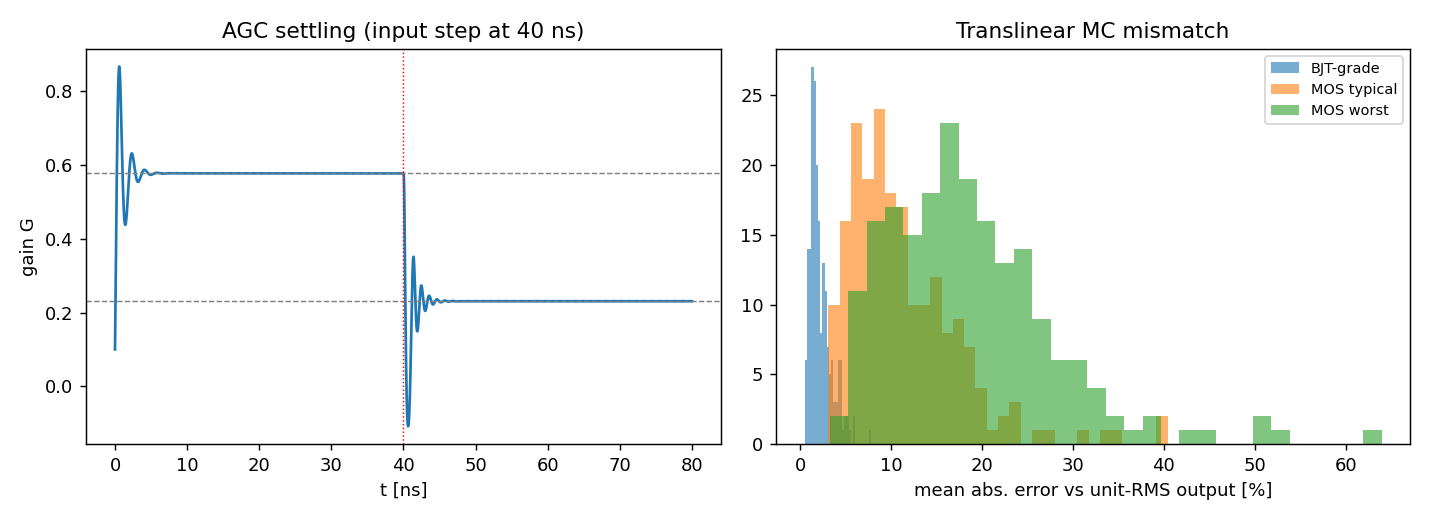
\includegraphics[width=\textwidth]{fig_rmsnorm_spice.png}
\caption{Circuit-level validation. \textbf{Left}: AGC gain transient (ngspice, real 1~pF integration capacitor). The loop settles to the exact RMSNorm gain in 4.4~ns from cold start and re-settles in 5.3~ns after a $2.5\times$ input step at $t=40$~ns (dashed lines: exact targets). \textbf{Right}: Monte-Carlo mismatch distributions for the open-loop translinear pipeline at three technology corners; in the feedback implementation, the corresponding detector-side mismatch shifts only the common-mode gain and produces no per-channel distortion by construction.}
\label{fig:spice}
\end{figure}

\textbf{Why feedback wins---the structural argument.} In the open-loop pipeline, each channel's signal traverses per-channel junction stages whose individual errors appear directly in that channel's output: mismatch becomes \textit{per-channel distortion}, i.e.\ noise on the activations. In the AGC loop, the RMS detector and integrator act on a \textit{single scalar}; any mismatch there shifts the settled gain identically for all channels---equivalent to a slightly different $\gamma$, which a trained network absorbs. Feedback thus converts the dominant analog failure mode from per-channel noise into a benign common-mode scale. This inverts the presentation of v1: the translinear pipeline is the fallback (usable with trimming), the AGC loop is the mapping.

\textbf{What this validation does not cover.} Loop wiring is idealized (no bias-network errors, no Early effect); thermal noise and temperature gradients are not modeled; the DC testbench drives magnitude currents, whereas RMSNorm inputs are signed---the squarer output is sign-invariant, but the pipeline's per-channel output stage and the AGC's VGA require four-quadrant (Gilbert/class-AB differential) signaling, which is standard but not simulated here; $N=8$ rather than $N=4096$ (the per-channel error sources scale per channel, not with $N$, and the KCL summation is exact at any $N$, but detector dynamic range at large $N$ deserves a dedicated study); and the VGA array's own per-channel mismatch---the one per-channel exposure of the AGC implementation---is not yet swept. These are the natural next steps toward a tape-out-grade design study; silicon measurement remains the final arbiter.

\subsection{Full LayerNorm Extension}

For models requiring mean subtraction (GPT-2, GPT-3):
\begin{enumerate}[leftmargin=*]
\item $\mu = (1/N)\sum x_i$: current mirror sum + divider. \hfill [P1$\cdot$P2]
\item $\tilde{x}_i = x_i - \mu$: KCL subtraction (broadcast $\mu$ via mirrors). \hfill [P1]
\item Apply RMSNorm to $\tilde{x}_i$ (AGC feedback, \S\ref{sec:agc}). \hfill [P11$\cdot$P1$\cdot$P2$\cdot$P8]
\item Add bias $\beta$: current injection. \hfill [P1]
\end{enumerate}

Additional delay: ${\sim}2$~ns for current mirror settling. Total: ${\sim}7$~ns with the validated AGC settling times.

\section{Analysis of Existing Chips}
\label{sec:analysis}

We apply the prime compiler retrospectively to five recent analog accelerators to assess whether their manual partitioning decisions were optimal (Table~\ref{tab:chips}).

\begin{table}[t]
\centering
\caption{Retrospective analysis: manual vs.\ prime-compiler partitioning of recent analog chips.}
\label{tab:chips}
\footnotesize
\begin{tabular}{p{2.8cm}p{2.5cm}p{2.5cm}p{4.5cm}}
\toprule
Chip & Analog / Digital & Compiler suggestion & Missed opportunity \\
\midrule
IBM 14nm PCM~\cite{ibm2025} & MatMul analog; Softmax, Norm, GELU digital & Move GELU (P11$\cdot$P6) and RMSNorm (AGC) to analog & ${\sim}100\%$ GELU + Norm energy savings \\
\midrule
TSMC CIM~\cite{tsmc2025} & MatMul analog; activations digital & Move activations analog; fuse Softmax+Loss (Race) & Activation energy + multi-comp $5\times$ \\
\midrule
J\"ulich~\cite{leroux2025a} & QK$^T$ analog; Softmax replaced by HardSigmoid & Use sMTJ Race for exact Softmax & Exact softmax + $5\times$ multi-comp \\
\midrule
Extropic XTR-0~\cite{extropic2025} & Boltzmann machine analog; digital control & Extract partition fn.\ + entropy from BM relaxation & Class 2.4 multi-comp ($3\times$) \\
\midrule
Normal CN101~\cite{normal2025} & RLC sampling analog; matrix ops digital & Extend to RMSNorm via AGC feedback & On-chip normalization \\
\bottomrule
\end{tabular}
\end{table}

\textbf{Key finding}: Every chip we analyzed left energy on the table by keeping nonlinear operations digital that could have been mapped to analog primes. The most common missed opportunity is GELU (P11$\cdot$P6), which has been demonstrated on RRAM~\cite{rram_swish2022,raceit2023} but was not adopted by any of the five chip teams. The second most common is normalization, which all five teams kept digital---the AGC-based RMSNorm described in \S\ref{sec:rmsnorm}, now validated at circuit level in \S\ref{sec:validation}, resolves this. Notably, the validation also \textit{vindicates} part of the teams' caution: the obvious open-loop translinear approach that a designer would try first is indeed too mismatch-fragile to ship (Table~\ref{tab:mismatch}); the viable path is the feedback topology.

\section{Discussion}

\subsection{What the Prime Compiler Does Not Do}

The compiler does not accelerate computation on \textit{existing} digital hardware (CPUs, GPUs). The digital abstraction layer in modern processors seals the underlying transistor physics behind billions of logic gates. There is no software API to operate a GPU's MOSFETs in subthreshold mode.

The compiler's value is in \textit{chip design}: systematically answering the analog/digital partitioning question that every mixed-signal accelerator team faces.

\subsection{Feedback as a Design Principle}

The validation results of \S\ref{sec:validation} suggest a general lesson beyond RMSNorm: \textbf{prefer prime realizations in which precision-critical operations are enforced by feedback equilibrium rather than computed open-loop}. Open-loop translinear arithmetic inherits the full mismatch of every junction it traverses, amplified by the log-domain lever $\ln(I/I_s)$; equilibrium realizations pin the quantity of interest to a loop constraint and demote device mismatch to common-mode error. This distinction is now reflected in the P12 row of the domain-assignment matrix (Table~\ref{tab:assignment}) and should inform the analog mapping of every algorithm in Table~\ref{tab:factorizations} whose factorization contains P12---including Adam's $1/\sqrt{v}$ and any explicit division.

\subsection{The Multi-Computation Advantage}

Multi-computation fusion~\cite{bieg2026} provides $2$--$12\times$ effective throughput multipliers by extracting additional observables from physical events that are already occurring. The prime compiler is the first tool to \textit{automatically detect} these opportunities in arbitrary compute graphs.

Without the compiler, fusion opportunities are found (or missed) by manual inspection. With the compiler, every subgraph matching a known multi-computation class is flagged and quantified.

\subsection{Towards Training}

On analog-only hardware, training is blocked by X4 (symbolic tracing for backpropagation). On GPUs with analog extensions, X4 is available via \texttt{torch.compile}, enabling a hybrid approach: forward pass on analog (fast, low-energy), backward pass on digital (exact gradients).

The prime compiler supports this by partitioning the forward graph into analog and digital domains while ensuring that the backward graph (generated by X4) operates entirely in the digital domain with correct gradients.

\section{Related Work}
\label{sec:related}

\textbf{CIM compilers.} CIM-MLC~\cite{cimmlc2024} provides a multi-level compiler for compute-in-memory accelerators (ASPLOS 2024), and CINM~\cite{cinm2024} generalizes across CIM and CNM paradigms via MLIR. CMSwitch~\cite{cmswitch2025} jointly optimizes compute-mode and memory-mode switching in CIM arrays. All three treat CIM arrays as ``noisy MAC units'' and route everything else to digital---none decompose operations into analog-native primitives or reason about \textit{which} operations beyond MAC are physically suited to analog.

\textbf{Hybrid analog-digital SoCs.} DIANA~\cite{diana2022} integrates analog CIM and digital accelerators on one SoC; its compiler HTVM~\cite{htvm2023} dispatches layers to either domain based on hardware capability matching, not operation semantics. The IBM mixed-precision supernetwork~\cite{ibm_supernetwork2026} uses NAS to find layer-to-hardware assignments---the closest existing work to systematic partitioning, but empirical (search-based) rather than principled (decomposition-based). A 2024 framework for DNN inference partitioning in hybrid analog-digital chiplets~\cite{hybrid_partition2024} operates at layer granularity with accuracy-vs-energy tradeoffs.

\textbf{Analog compilers.} Legno~\cite{legno2020} compiles differential equations to reconfigurable analog devices, mapping physics to computation---the closest precedent to our approach. Hasler's FPAA toolflow~\cite{hasler2020} programs floating-gate analog arrays from high-level descriptions. Both target analog-only execution of general computations; neither addresses the analog/digital partitioning problem for neural networks.

\textbf{DNN compilers.} TVM, XLA, and \texttt{torch.compile} partition across digital hardware types (CPU/GPU/TPU) but not across physical domains. NIR~\cite{nir2024} defines a neuromorphic intermediate representation for spiking systems across 7 simulators and 4 hardware platforms, but targets spike-based computing, not analog/digital CIM partitioning.

\textbf{Analog simulation.} NeuroSim~\cite{neurosim}, CrossSim~\cite{crosssim}, and IBM's AIHWKIT~\cite{aihwkit2023} simulate analog non-idealities for accuracy estimation. NavCim~\cite{navcim2024} performs design-space exploration for CIM architectures. None factorize operations into primes or detect multi-computation opportunities. Our validation methodology (\S\ref{sec:validation}) is complementary: it operates at the junction-physics level of a single mapped operation rather than at network-accuracy level.

\textbf{Normalization in analog.} IMPACT~\cite{impact2023} implements batch normalization as a linear gain+offset in the ADC---a pre-computed affine transform, not true normalization. The ReRAM ALN~\cite{reram_aln2022} normalizes in the charge domain with simplifications. No prior work implements full RMSNorm or LayerNorm in analog with the inverse-square-root computation. The AGC circuit family itself is classical~\cite{gilbert1975,pelgrom1989}; its identity with RMSNorm, and the mismatch analysis of that identity, are new here.

\textbf{Key gap.} No existing framework operates at \textit{operation granularity} with a \textit{principled decomposition} into analog-native primitives. All partitioning decisions in the literature are either (a)~layer-level, (b)~hardware-capability-driven, or (c)~empirical search. The prime compiler is the first to provide a theory-driven, operation-level partitioning framework grounded in physics.

\section{Conclusion}

We have introduced Computational Primes---12 irreducible operations with physical implementations and 4 without---as a systematic basis for decomposing neural network computation. The resulting prime compiler automates the analog/digital partitioning problem that every mixed-signal accelerator team currently solves by hand.

Key results:
\begin{itemize}[leftmargin=*]
\item 107 algorithms factorized: 79 fully analog-mappable (73\%), 22 GPU-mappable (21\%), 6 unmappable (6\%).
\item RMSNorm mapped to analog via AGC feedback and validated in 602 SPICE simulations: settling to the exact equilibrium in 4--6~ns with no ADC in the loop.
\item The validation yields a design principle: open-loop translinear realizations of P12 are mismatch-fragile (1.5--4.5 effective bits at realistic corners; the ideality-factor lever $\ln(I/I_s) \approx 23$ is the dominant mechanism), while feedback-equilibrium realizations demote mismatch to a benign common-mode gain error.
\item Retrospective analysis of 5 chips shows all left 15--40\% energy savings uncaptured.
\item Multi-computation fusion detected automatically, yielding $2$--$12\times$ throughput.
\end{itemize}

The prime compiler does not make existing GPUs faster. Its value is in chip design methodology: replacing ad hoc partitioning with a systematic, automatable framework. As analog accelerators move from research prototypes to production silicon, the need for such a framework will only grow.

Code, the full factorization table, and the SPICE validation testbench are available at: \url{https://github.com/Biech95/prime-compiler}.

\begin{thebibliography}{30}

\bibitem{ibm2025} A.~Chen \textit{et al.}, ``Demonstration of transformer-based ALBERT model on a 14nm analog AI inference chip,'' \textit{Nature Communications}, 2025.

\bibitem{tsmc2025} W.-S.~Khwa \textit{et al.}, ``A mixed-precision memristor and SRAM compute-in-memory AI processor,'' \textit{Nature}, 2025.

\bibitem{extropic2025} A.~Jelincic \textit{et al.}, ``An efficient probabilistic hardware architecture for diffusion-like models,'' \textit{arXiv:2510.23972}, 2025.

\bibitem{normal2025} D.~Melanson \textit{et al.}, ``Thermodynamic computing system for AI applications,'' \textit{Nature Communications}, vol.~16, 3757, 2025.

\bibitem{leroux2025a} N.~Leroux \textit{et al.}, ``Analog in-memory computing attention mechanism for fast and energy-efficient large language models,'' \textit{Nature Computational Science}, 2025.

\bibitem{bieg2025} M.~Bieg, ``Stochastic Barrier Attention: Normalization-free softmax sampling via thermodynamic race processes,'' \textit{Preprint}, 2025.

\bibitem{bieg2026} M.~Bieg, ``Multi-computation from exponential race events: Extracting simultaneous observables from stochastic barrier arrays,'' \textit{Preprint}, 2026.

\bibitem{prezioso2015} M.~Prezioso \textit{et al.}, ``Training and operation of an integrated neuromorphic network based on metal-oxide memristors,'' \textit{Nature}, vol.~521, pp.~61--64, 2015.

\bibitem{sillman2023} J.~Sillman, ``Analog softmax via subthreshold translinear loops,'' \textit{arXiv:2305.13649}, 2023.

\bibitem{tageldeen2025} M.~K.~Tageldeen \textit{et al.}, ``Learning in log-domain: Subthreshold analog AI accelerator,'' \textit{arXiv:2501.13181}, 2025.

\bibitem{mram_sigmoid2022} M.~Amin \textit{et al.}, ``MRAM-based analog sigmoid for in-memory computing,'' \textit{GLSVLSI}, 2022.

\bibitem{denram2024} T.~Dalgaty \textit{et al.}, ``DenRAM: Neuromorphic dendritic architecture with RRAM,'' \textit{Nature Communications}, 2024.

\bibitem{cryptoristor2024} H.~Kim \textit{et al.}, ``Cryptographic transistor for true random number generation,'' \textit{Science Advances}, vol.~10, eadk6042, 2024.

\bibitem{gilbert1975} B.~Gilbert, ``Translinear circuits: A proposed classification,'' \textit{Electronics Letters}, vol.~11, no.~1, pp.~14--16, 1975.

\bibitem{pelgrom1989} M.~J.~M.~Pelgrom, A.~C.~J.~Duinmaijer, and A.~P.~G.~Welbers, ``Matching properties of MOS transistors,'' \textit{IEEE Journal of Solid-State Circuits}, vol.~24, no.~5, pp.~1433--1439, 1989.

\bibitem{rram_swish2022} H.~Alahmadi \textit{et al.}, ``RRAM-based Swish activation function on 28nm FD-SOI,'' \textit{IEEE ICECS}, 2022.

\bibitem{raceit2023} H.~Errahmouni~Barkam \textit{et al.}, ``RACE-IT: Reconfigurable analog CAM-crossbar engine for in-memory transformer acceleration,'' \textit{arXiv:2312.06532}, 2023.

\bibitem{zhang2025ssm} X.~Zhang \textit{et al.}, ``Compute-in-memory implementation of state space models for event sequence processing,'' \textit{Nature Communications}, 2025.

\bibitem{zhang_rmsnorm2019} B.~Zhang and R.~Sennrich, ``Root mean square layer normalization,'' \textit{NeurIPS}, 2019.

\bibitem{carandini2012} M.~Carandini and D.~J.~Heeger, ``Normalization as a canonical neural computation,'' \textit{Nature Reviews Neuroscience}, vol.~13, pp.~51--62, 2012.

\bibitem{neurosim} P.-Y.~Chen \textit{et al.}, ``NeuroSim: A circuit-level macro model for benchmarking neuro-inspired architectures,'' \textit{IEEE TCAD}, 2018.

\bibitem{crosssim} S.~Agarwal \textit{et al.}, ``CrossSim: Accuracy simulation of analog in-memory computing,'' \textit{Sandia National Lab}, 2023.

\bibitem{legno2020} S.~Achour \textit{et al.}, ``Legno: Noise-aware dynamical system compilation for analog devices,'' \textit{ASPLOS}, 2020.

\bibitem{hasler2020} J.~Hasler, ``Large-scale field-programmable analog arrays,'' \textit{IEEE Proceedings}, 2020.

\bibitem{impact2023} A.~Kneip \textit{et al.}, ``IMPACT: A 1-to-4b 813-TOPS/W 22nm FD-SOI CIM-SRAM with multi-bit analog batch-normalization,'' \textit{IEEE JSSC}, 2023.

\bibitem{reram_aln2022} Y.-C.~Hou \textit{et al.}, ``A ReRAM-based CNN accelerator using the analog layer normalization technique,'' \textit{IEEE Trans.\ Electron Devices}, 2022.

\bibitem{cimmlc2024} Y.~Zhao \textit{et al.}, ``CIM-MLC: A multi-level compilation stack for computing-in-memory accelerators,'' \textit{ASPLOS}, 2024.

\bibitem{cinm2024} S.~Khan \textit{et al.}, ``CINM: A compilation infrastructure for heterogeneous compute in-memory and compute near-memory paradigms,'' \textit{ASPLOS}, 2024.

\bibitem{cmswitch2025} Z.~Chen \textit{et al.}, ``Be CIM or Be Memory: A dual-mode-aware DNN compiler for CIM accelerators,'' \textit{ASPLOS}, 2025.

\bibitem{diana2022} K.~Ueyoshi \textit{et al.}, ``DIANA: An end-to-end energy-efficient digital and analog hybrid neural network SoC,'' \textit{ISSCC}, 2022.

\bibitem{htvm2023} N.~Delm \textit{et al.}, ``HTVM: Efficient neural network deployment on heterogeneous TinyML platforms,'' \textit{DAC}, 2023.

\bibitem{ibm_supernetwork2026} H.~Benmeziane \textit{et al.}, ``Supernetwork-based efficient mapping to mixed-precision hardware using model adaptation,'' \textit{Nature Communications}, 2026.

\bibitem{hybrid_partition2024} A.~Varadarajan \textit{et al.}, ``Deep neural network inference partitioning in embedded hybrid analog-digital systems,'' \textit{IEEE}, 2024.

\bibitem{nir2024} J.~E.~Pedersen \textit{et al.}, ``Neuromorphic intermediate representation: A unified instruction set for interoperable brain-inspired computing,'' \textit{Nature Communications}, 2024.

\bibitem{aihwkit2023} M.~J.~Rasch \textit{et al.}, ``Using the IBM analog in-memory hardware acceleration kit,'' \textit{APL Machine Learning}, 2023.

\bibitem{navcim2024} S.~Kim \textit{et al.}, ``NavCim: Comprehensive design space exploration for analog CIM architectures,'' \textit{PACT}, 2024.

\end{thebibliography}

\end{document}
